\section{Model evaluation}

Before analysing the mechanisms driving marine ecosystem response to ENSO variability, the physical, biogeochemical and biological models are evaluated against observation-based estimates.

\subsection{Physical and biogeochemical model}

Although successfully used in a variety of ENSO-related physical and biogeochemical studies in the tropical Pacific (e.g., \citealt{vialardModelStudyOceanic2001, lengaigneOceanResponseMarch2002, lengaigneInfluenceOceanicBiology2007, schneiderClimateinducedInterannualVariability2008, masottiLargescaleShiftsPhytoplankton2011, currieIndianOceanDipole2013}), the ability of our simulation to capture ENSO surface temperature, sea-level anomalies and chlorophyll signature is briefly evaluated. 

This ability is assessed by comparing observation-based and simulated covariance maps of detrended monthly anomalies with the Oceanic Nino Index\footnote{\url{https://www.cpc.ncep.noaa.gov/data/indices/oni.ascii.txt}} (hereafter ONI), which is the NOAA official ENSO indicator. It is based on a 3-month running mean of sea-surface tegeosmperature anomalies averaged over the Niño 3.4 region (5N-5S, 170W-120W).

\subsubsection{Sea-surface temperature}
\label{sec:sst}

As a first evaluation of the simulated sea-surfate temperature, the simulated ONI index is compared with the one provided by the NOAA (Fig\ref{fig:nemo-had-sst}a). The two time-series show a strong correlation of 0.92 over their common 1958-2018 period. In particular, the model is able to accurately capture the timing and amplitude of major El Niño events, like in 1972/73, 1982/83, 1997/98 and 2015/16 and of major La Niña events, like in 1988/89 and 1999/2000. 

As a second evaluation, the spatial structure of simulated sea-surface temperature response to ENSO is compared with the one obtained with the Hadley Sea-Surface Temperature dataset\footnote{\url{https://www.metoffice.gov.uk/hadobs/hadisst/data/download.html}} (HadISST1, \citealt{raynerGlobalAnalysesSea2003}). HadISST1 uses reduced space optimal interpolation applied to SSTs from the Marine Data Bank (mainly ship tracks) and ICOADS through 1981 and a blend of in-situ and adjusted satellite-derived SSTs for 1982-onwards. The resulting dataset is provided as monthly sea-surface temperature maps on a $1\times 1$ regular grid. The covariances obtained with the HadISST1 anomalies and the simulated ones are shown in Fig.\ref{fig:nemo-had-sst}b and Fig.\ref{fig:nemo-had-sst}c.

\begin{figure}[htp]
	\centering
	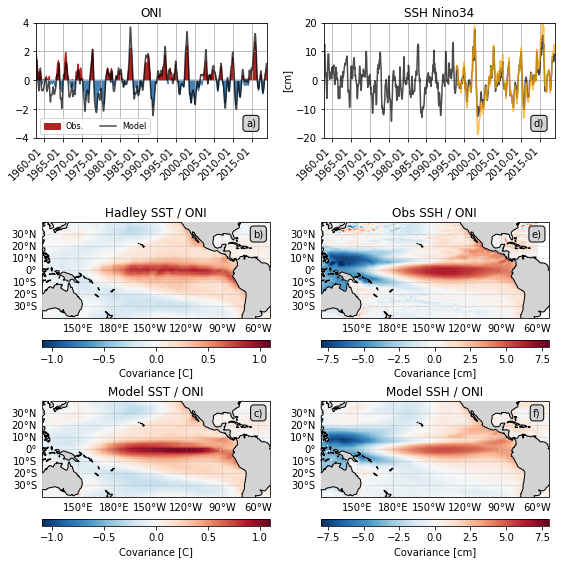
\includegraphics[scale=0.6]{figs/fig1.png}
	\caption{Observed and simulated ONI indexes (a). Covariance between the ONI index and the Hadley (b) and simulated SST anomalies (c). Observed and simulated sea-level anomalies averaged over the Nino34 region (d). Covariances between the ONI index and the observed (e) and simulated (f) sea-level anomalies. The dashed box represents the Nino34 region.}
	\label{fig:nemo-had-sst}
\end{figure}

Simulated ENSO SST  pattern closely resembles the observed one. This pattern is characterized by warm SST anomalies (1\degree{}C) centred in the central and eastern equatorial Pacific  flanked by the traditional horseshoe cooling pattern in the western Pacific extending towards the subtropical north and south Pacific. This SST seesaw in the equatorial region is further accompanied by a shoaling of the thermocline in the west and a deepening in the east, which can be inferred from sea-level anomalies.

\subsubsection{Sea-level anomalies}

Simulated sea-level anomalies are compared with the reprocessed Global Ocean Gridded L4 Sea-Surface Heights\footnote{\url{https://doi.org/10.48670/moi-00148}} data, provided by the Copernicus Climate Service as monthly values on a regular $0.25 \times 0.25$ grid from 1993-01 to 2020-12. This product was built by the DUACS multimission altimeter data processing system, which processes data from all altimeter missions: Jason-3, Sentinel-3A, HY-2A, Saral/AltiKa, Cryosat-2, Jason-2, Jason-1, T/P, ENVISAT, GFO, ERS1/2. Using along-track altimeter data, gridded sea-level anomalies are extracted by using an Optimal Interpolation off all the flying satellites. 

The simulated sea-level anomalies averaged over the Nino34 region compare well with the observed ones (Fig \ref{fig:nemo-had-sst}d), with a correlation coefficient of 0.94. In addition, the spatial patterns associated with ENSO variability are very similar for both the observations and the model (Fig \ref{fig:nemo-had-sst}e, Fig \ref{fig:nemo-had-sst}f). Sea-level anomalies are negative in the western Pacific and positive in the central and eastern Pacific. These anomalies are consistent with thermocline vertical displacements, which shoal in the west and deepens in the east (\warn{REF}).

\subsubsection{Chlorophyll}

Simulated chlorophyll has been compared with observation-based estimates extracted from the monthly OceanColour-CCI V5 CHL-a dataset\footnote{\url{http://dx.doi.org/10.5285/1dbe7a109c0244aaad713e078fd3059a}} \citep{sathyendranathOceanColourTimeSeries2019} over the 1997-09/2018-12 period. The high resolution (4 km)  dataset has been regridded on a regular $1\times 1$ grid by computing weighted chlorophyll averages over $24\times24$ boxes, with the weights being provided by the cosine of latitude. When more than $1/3$ of the data used in the averaging is missing, the regridded cell is masked.

Covariance maps between the surface chlorophyll and the monthly ONI index, computed over the common period, are shown in Fig \ref{fig:nemo-sat-chl}. The observations (upper panel) and the model (lower panel) show very similar covariance patterns: El Nino induces a decrease in chlorophyll concentration along the equator east of 150\degree{}E, consistent with a weaker equatorial upwelling induced by the equatorial trade winds reduction. However, the model overestimates the chlorophyll response to ENSO variability compared with observational based estimates. Note that the covariance for the simulated chlorophyll has also been computed over the entire simulated period (1958-2018), with no significant changes in the resulting pattern (not shown). 

The observed and simulated chlorophyll anomalies, averaged along the equatorial band, have a correlation coefficient of $0.80$.

\begin{figure}[htp]
	\centering
	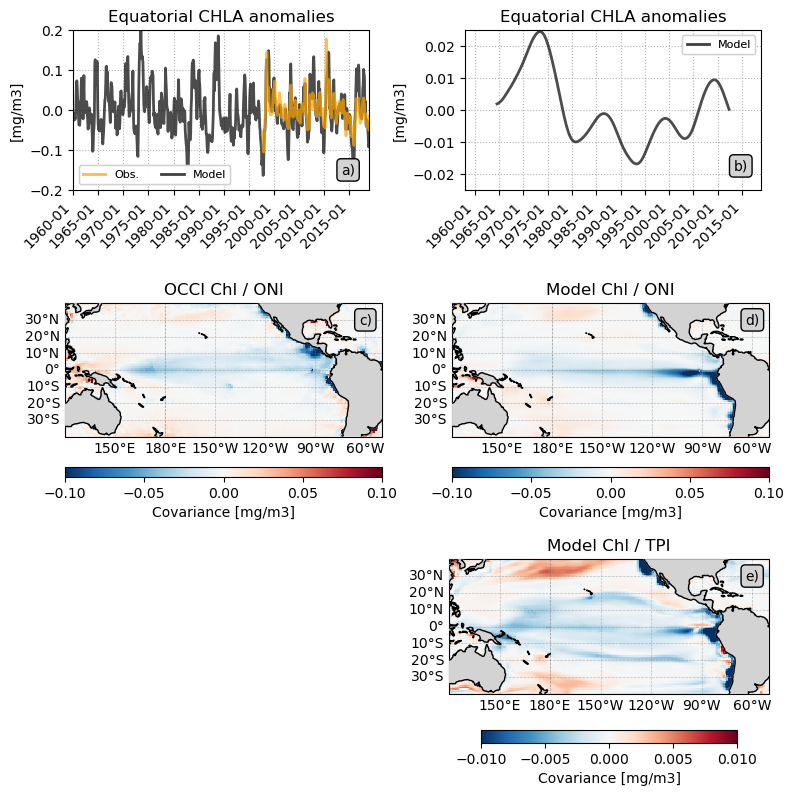
\includegraphics[scale=0.4]{figs/fig2.png}
	\caption{Simulated (black) and observed (yellow) equatorial chlorophyll anomalies (a). Filtered anomalies are shown for the model in panel (b). Covariance between the observed and simulated chlorophyll anomalies with the ONI (c, d) and filtered TPI (e) index. The dashed box represents the equatorial region used in the averaging.}
	\label{fig:nemo-sat-chl}
\end{figure}

\subsection{Marine ecosystem model}

Before analysing the mechanisms of fish biomass response to El Nino variability, simulated biomass integrated from 30cm to 70cm is compared with the observation-based estimates extracted from the IRD Level 2 global monthly catch of tuna, tuna-like and shark species dataset\footnote{\url{https://doi.org/10.5281/zenodo.1164128}} \citep{taconetGlobalMonthlyCatch2018}. First, the purse-seine captures of skipjack and yellowfin tunas have been extracted from the raw input file. Then, non-monthly observations (i.e. when the difference between the end and start dates exceed 31 days) have been discarded, as well as those which are unlocalized. Finally, the remaining observations have been regridded into on a regular $1 \times 1$ grid using the overlapping area between the observation polygon and the destination cell. The final product is a $3D$ array of dimensions (time and space) that extends from 1959 to 2016. However, due to the early poor data coverage, this dataset was used from 1985 onward.

Figure \ref{fig:apecosm_validation}a shows the Hovmoller diagram of the observed catches and fish biomass (log-scale) integrated between 10N and 10S for the 2008-2018 period. Although observed and model results cannot be directly compared, some features are well captured by the model. For instance, the easternmost $4.00$ simulated contour seems to closely follow the eastward extensions of catches that occur in 2010, 2012 and 2016. Figure \ref{fig:apecosm_validation}b shows, for a longer period (1985-2018), the longitudinal position of the catch and biomass barycenters. The observed barycenter shows an eastward trend, liley due to the increased power of fishing fleets, which allow them to navigate over greater distances from their fishing ports, mostly located in the western Pacific (\warn{ref}). This emphasizes the fact that the data used in this validation are catch data, which are not only dependent on fish biomass but also depend on fishing effort, and as such must be used with caution for the comparison with simulated fish biomass. Figures \ref{fig:apecosm_validation}c and \ref{fig:apecosm_validation}d show the difference between catch and simulated biomass composites for El Nino (OND2009-JFM2010, OND2014-JFM2015, OND-2015-JFM2016) and La Nina conditions (OND2007-JFM2008, OND2008-JFM2009, OND2010-JFM2011, OND2011-JFM2012). Observed catches increase in the central and eastern Pacific and decrease in the Western Pacific when switching from La Nina to El Nino conditions, which is consistent with an eastward displacement of the fish biomass. Simulated composite also shows an increase in the central Pacific and a decrease in the west, although the pattern seems westward shifted compared with the catch composite. 

\begin{figure}[htp]
	\centering
	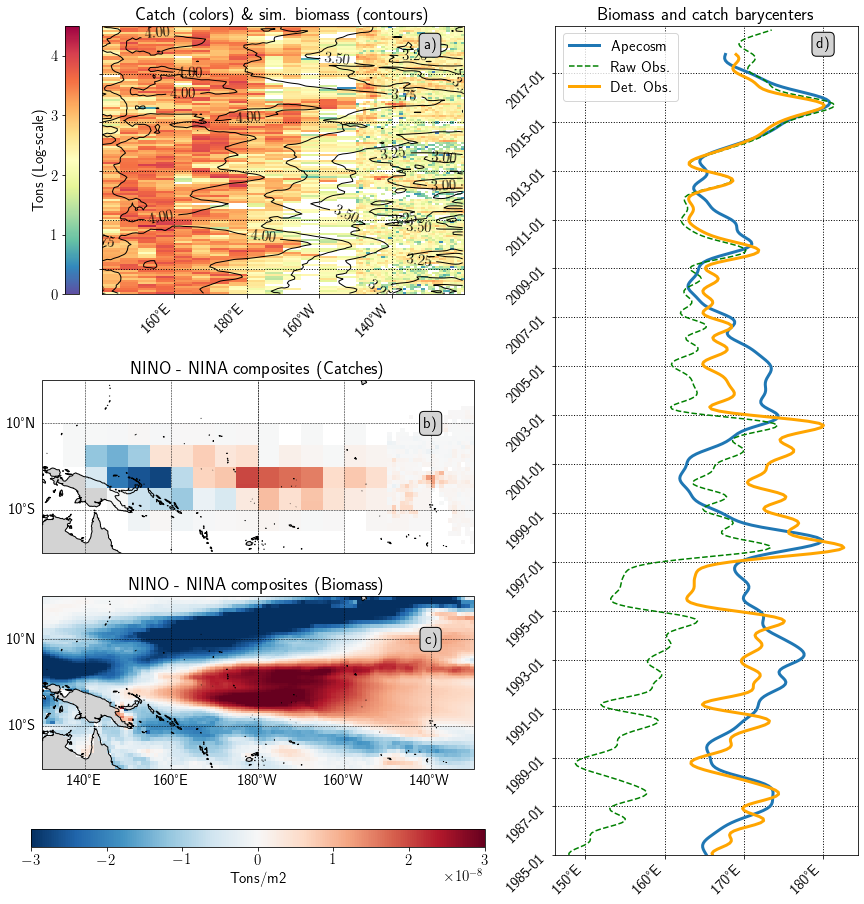
\includegraphics[scale=0.35]{figs/plot_validation_apecosm.png}
	\caption{Hovmoller diagram of observed catches (colors) and simulated fish biomass (contours) integrated between 10N and 10S (a, log-scale) and associated barycenters (b). Catch (c) and simulated fish-biomass (d) difference between El Nino and La Nina composites.}
	\label{fig:apecosm_validation}
\end{figure}

In the following, the results for three size classes, 3cm, representing small fishes, 20cm, representing intermediate sizes, and 90 cm, representing large individuals, will be detailed. The latter are representative of the sizes of tuna target species within the region (\warn{REF}). \\

%\clearpage